\begin{center}
    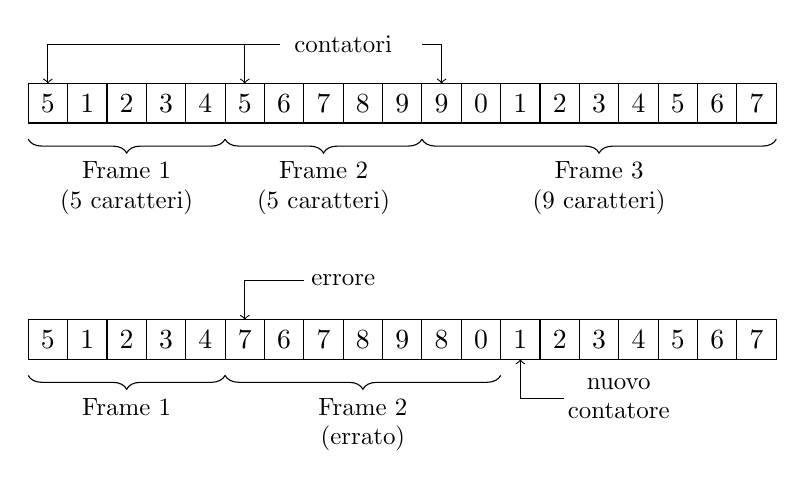
\begin{tikzpicture}
        %%%%%%%% Blocchi %%%%%%%%%
        \foreach \x in {0,0.5,...,9}
            \draw (\x,0) rectangle ([shift={(\x,0)}] 0.5,0.5);

        \foreach \x in {0,0.5,...,9}
            \draw (\x,3) rectangle ([shift={(\x,0)}] 0.5,3.5);

        %%%%%%%%% Numeri %%%%%%%%%
        \node at (0.25,0.25) {5};
        \node at (0.75,0.25) {1};
        \node at (1.25,0.25) {2};
        \node at (1.75,0.25) {3};
        \node at (2.25,0.25) {4};
        \node at (2.75,0.25) {7};
        \node at (3.25,0.25) {6};
        \node at (3.75,0.25) {7};
        \node at (4.25,0.25) {8};
        \node at (4.75,0.25) {9};
        \node at (5.25,0.25) {8};
        \node at (5.75,0.25) {0};
        \node at (6.25,0.25) {1};
        \node at (6.75,0.25) {2};
        \node at (7.25,0.25) {3};
        \node at (7.75,0.25) {4};
        \node at (8.25,0.25) {5};
        \node at (8.75,0.25) {6};
        \node at (9.25,0.25) {7};
        \node at (0.25,3.25) {5};
        \node at (0.75,3.25) {1};
        \node at (1.25,3.25) {2};
        \node at (1.75,3.25) {3};
        \node at (2.25,3.25) {4};
        \node at (2.75,3.25) {5};
        \node at (3.25,3.25) {6};
        \node at (3.75,3.25) {7};
        \node at (4.25,3.25) {8};
        \node at (4.75,3.25) {9};
        \node at (5.25,3.25) {9};
        \node at (5.75,3.25) {0};
        \node at (6.25,3.25) {1};
        \node at (6.75,3.25) {2};
        \node at (7.25,3.25) {3};
        \node at (7.75,3.25) {4};
        \node at (8.25,3.25) {5};
        \node at (8.75,3.25) {6};
        \node at (9.25,3.25) {7};
        
        %%%%%% Decorations %%%%%%%
        \node[scale=0.9] at (4,1) {errore};
        \node[align=center,scale=0.9] at (7.5,-0.5) {nuovo\\contatore};
        \node[scale=0.9] at (4,4) {contatori};
        
        %%%%%%%%% Frecce %%%%%%%%%
        \draw[->] (3.5,1) -- (2.75,1) -- (2.75,0.5);
        \draw[->] (6.8,-0.5) -- (6.25,-0.5) -- (6.25,-0);
        \draw[->] (3.2,4) -- (0.25,4) -- (0.25,3.5);
        \draw[->] (2.75,4) -- (2.75,3.5);
        \draw[->] (5,4) -- (5.25,4) -- (5.25,3.5);

        %%%%%%%%% Graffe %%%%%%%%%
        \draw [decorate,decoration={brace,amplitude=5pt,mirror,raise=4ex}] (0,0.4) -- (2.5,0.4) node[scale=0.9,midway,yshift=-3.2em]{Frame 1};
        \draw [decorate,decoration={brace,amplitude=5pt,mirror,raise=4ex}] (2.5,0.4) -- (6,0.4) node[align=center,midway,yshift=-3.5em,scale=0.9]{Frame 2\\(errato)};
        \draw [decorate,decoration={brace,amplitude=5pt,mirror,raise=4ex}] (0,3.4) -- (2.5,3.4) node[align=center,midway,yshift=-3.5em,scale=0.9]{Frame 1\\(5 caratteri)};
        \draw [decorate,decoration={brace,amplitude=5pt,mirror,raise=4ex}] (2.5,3.4) -- (5,3.4) node[align=center,midway,yshift=-3.5em,scale=0.9]{Frame 2\\(5 caratteri)};
        \draw [decorate,decoration={brace,amplitude=5pt,mirror,raise=4ex}] (5,3.4) -- (9.5,3.4) node[align=center,midway,yshift=-3.5em,scale=0.9]{Frame 3\\(9 caratteri)};
    \end{tikzpicture}
\end{center}